\documentclass[10pt]{article}
\usepackage[margin=0.72in]{geometry}
\usepackage[T1]{fontenc}
\usepackage{lmodern}
\usepackage{microtype}
\usepackage{graphicx}
\usepackage{booktabs}
\usepackage{tabularx}
\usepackage{longtable}
\usepackage{array}
\usepackage{amsmath}
\usepackage{amssymb}
\usepackage[table]{xcolor}
\usepackage{enumitem}
\usepackage{xurl}
\usepackage{hyperref}
\usepackage{caption}
\usepackage{placeins}
\usepackage{float}
\hypersetup{colorlinks=true,linkcolor=blue!55!black,urlcolor=blue!55!black,citecolor=blue!55!black}
\graphicspath{{figures/}}
\setlength{\parskip}{0.38em}
\setlength{\parindent}{0pt}
\setlength{\emergencystretch}{1em}
\renewcommand{\arraystretch}{1.08}
\captionsetup{font=small,labelfont=bf,justification=raggedright,singlelinecheck=false}
\newcommand{\pp}{\,\mathrm{pp}}
\newcommand{\ci}[2]{[#1,\,#2]}
\newcommand{\compacttable}{\footnotesize\setlength{\tabcolsep}{3pt}\renewcommand{\arraystretch}{1.08}}
\definecolor{ResearchTeal}{HTML}{238B8E}
\definecolor{ResearchRed}{HTML}{B45C63}
\definecolor{ResearchMuted}{HTML}{64758A}
\definecolor{AblGoodLight}{HTML}{EAF3F2}
\definecolor{AblGoodMid}{HTML}{CDE4E1}
\definecolor{AblGoodDeep}{HTML}{A7CFCA}
\definecolor{AblBadLight}{HTML}{F8EEEE}
\definecolor{AblBadMid}{HTML}{EFD8DA}
\definecolor{AblBadDeep}{HTML}{E3B9BC}
\newcommand{\present}{\textcolor{ResearchTeal}{\ensuremath{\checkmark}}}
\newcommand{\gain}[1]{\textcolor{ResearchTeal}{#1}}
\newcommand{\loss}[1]{\textcolor{ResearchRed}{#1}}
\newcommand{\humanicon}{\raisebox{-.08em}{
\includegraphics[height=.85em]{mode-human.pdf}}}
\newcommand{\agenticon}{\raisebox{-.08em}{
\includegraphics[height=.85em]{mode-agent.pdf}}}
\newcommand{\humancount}[1]{\mbox{#1\,\humanicon}}
\newcommand{\agentcount}[1]{\mbox{#1\,\agenticon}}
\newcommand{\mixedcounts}[2]{\mbox{\agentcount{#2}\,+\,\humancount{#1}}}
\newcommand{\mixedmodes}{\mbox{A\,\agenticon\,+\,H\,\humanicon}}
\newcolumntype{Y}{>{\raggedright\arraybackslash}X}

\title{When the Logs Change, Do Links Hold?\\
\large Same-Challenge Retrieval Across Human/Agent Mixtures}
\author{\raisebox{-0.3em}{
\includegraphics[height=1.35em,trim=70bp 33bp 65bp 32bp,clip]{attackagent-owl.png}}\hspace{0.45em}AttackAgent Detect}
\date{6 November 2026}

\begin{document}
\maketitle

\begin{abstract}
Mixed Human/Agent logs create a practical retrieval tension: thresholds that avoid false links can miss same-task candidates, while thresholds that recover them can accept unrelated traces. We test how this balance shifts as gallery role composition changes and whether local-behavior and sequence features (B/S) add beyond command evidence; same-challenge labels are retrieval proxies, not activity labels. An observation-aware, fold-adaptive pipeline selects available features and model settings inside task-disjoint training folds, then freezes them for held-out evaluation. Across 17 CTH tasks, raising the Agent share from 0\% to 100\% lowers action-bigram FMR by 23.09 percentage points and raises FSR by 44.93; Hit@1 is nearly unchanged and the 11.48-point gallery-AUC decline is uncertain. The primary matched CTH analysis finds no common B/S gain across three learners. A post-hoc XGBoost diagnostic shows a conditional +6.25-point BA increment with broader training-pair support and value-redacted arguments, but its multiplicity-adjusted interval includes zero. In frozen NYU Agent-only retrieval, XGBoost improves ranking and BA but FMR reaches 25.39\%; the tree's BA gain accompanies worse ranking, and SVM loses 8.23 BA points. AIT's measured T1--T6 increment is uncertain; T7--T8 are unavailable.
\end{abstract}

\section{Introduction}
Commands such as \texttt{pwd}, \texttt{ls}, and \texttt{grep} recur in unrelated sessions, while different runs of the same task can leave visibly different logs. A permissive matcher risks false merges; a cautious threshold misses same-task links. Retained logs often preserve commands and action order but omit the richer provenance or causal context used by event-correlation systems~\cite{holmes,poirot,atlas,ostinato}.

Figure~\ref{fig:architecture} previews the two readouts: recorded-mode estimation and trace-pair association. The pipeline adapts to the fields a source actually records, then selects its representation and model settings within task-disjoint training folds. Each selected configuration is frozen before scoring held-out tasks: this is nested, training-time adaptation, not online updating during an investigation.

\begin{figure}[H]
\centering
\resizebox{.84\linewidth}{!}{%
\begin{minipage}{\linewidth}
\centering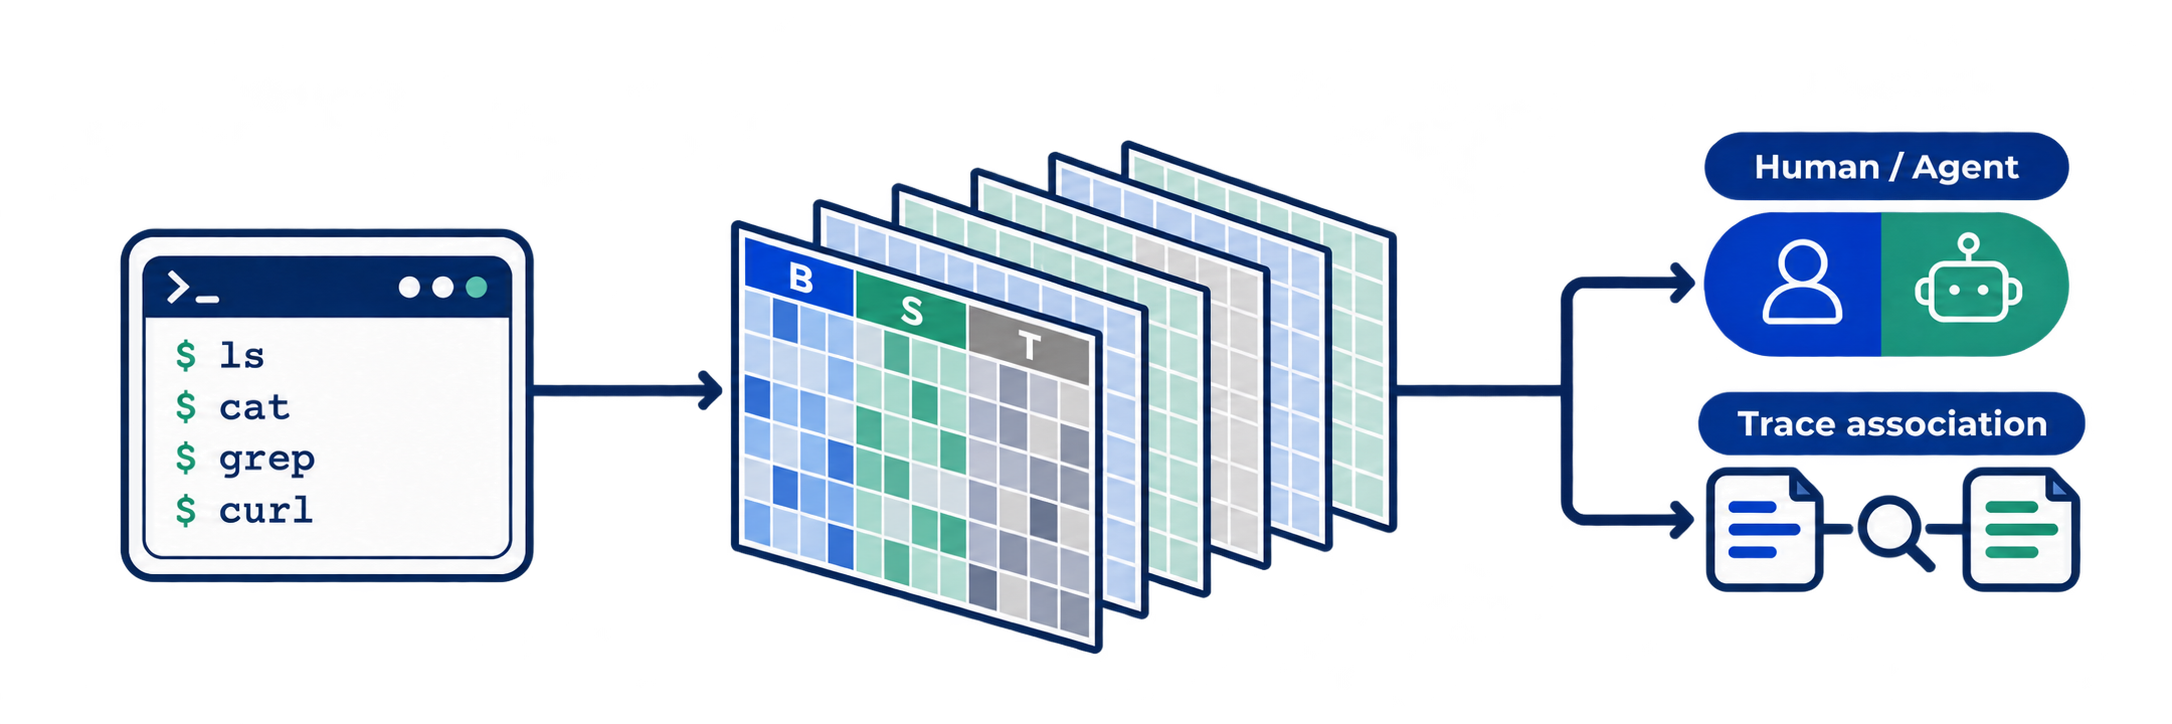
\includegraphics[width=\linewidth]{fingerprint-v3-overview.png}
\par\vspace{.15em}
\noindent\makebox[\linewidth][l]{%
\begin{minipage}[t]{.31\linewidth}\centering\small
\textbf{Observable logs}\\Commands, order, available time
\end{minipage}%
\begin{minipage}[t]{.38\linewidth}\centering\small
\textbf{Fold-adaptive B/S/T}\\Available blocks, window, fusion
\end{minipage}%
\hspace{.09\linewidth}%
\begin{minipage}[t]{.22\linewidth}\centering\small
\textbf{Two readouts}\\Mode estimates and trace links
\end{minipage}%
}\par
\end{minipage}%
}
\caption{Study design. Observable logs feed a fold-adaptive windowed fingerprint and two separately evaluated readouts. Inner task folds select settings; held-out tasks are reserved for evaluation. Timing remains missing when unobserved; displayed fields and values are illustrative.}
\label{fig:architecture}
\end{figure}

As AI agents become configurable participants in cyber operations, behavioral resemblance is increasingly easy to observe and easy to overinterpret. Synthetic APTs configured one model as five threat-group personas and reported partially convergent behaviors across profiles~\cite{syntheticapt}; it did not compare Human and Agent execution. We ask the narrower retrieval question: does recorded role composition change whether traces from the same benchmark task are linked? A \emph{false split} rejects a same-task pair, while a \emph{false merge} accepts a different-task pair. Benchmark-task identity is a retrieval proxy, not ground truth for shared activity or actor identity.

We use CTH to vary gallery composition, AIT to assess observed launch-gap timing, and NYU D-CIPHER to test external Agent-only retrieval. Across 17 CTH tasks, the fixed action-bigram threshold shifts from false merges toward missed links as the Agent share rises; Hit@1 is nearly unchanged and the gallery-AUC decline remains uncertain. The primary matched comparison finds no common B/S gain across learners. A post-hoc XGBoost diagnostic with broader training-pair support and value-redacted arguments gives a favorable point estimate, but its multiplicity-adjusted interval includes zero. NYU results show learner-specific ranking and error trade-offs. \textcolor{ResearchTeal}{\textbf{Association decisions depend on both the evidence in each trace and the Human/Agent mix of the candidate gallery.}} Our observation-aware, fold-adaptive framework makes these factors measurable by selecting available evidence and training-fold configurations, then reporting candidate ranking alongside both link errors. The current labels support same-challenge retrieval; they do not establish shared attack activity or actor identity.

\FloatBarrier
\section{Related work}
\subsection{System identity and workflow} Our question is whether already-collected traces can support candidate retrieval when the target relation is a shared benchmark task. This differs from identifying the model behind a trace or characterizing an Agent's preferred behavior. Prior work shows that terminal, coding, and browser actions can carry system-specific signals: Trace classifies model families from terminal commands; LIDAR actively probes coding agents; Known By Their Actions identifies browser models from UI events; and ProcGrep represents coding trajectories as procedures~\cite{trace,lidar,known,procgrep}. These readouts motivate log-derived features, while leaving same-task pair retrieval under changing Human/Agent composition as a distinct question.

\subsection{Cyber-agent behavior and relation labels} CyBiasBench is especially relevant to Agent profiling: its 630 sessions and request-level HTTP traces carry Agent, target, and attack-family labels, supporting Agent-side profile analysis and target-held-out evaluation~\cite{cybias}. Its public cohort has no Human traces and its HTTP request view differs from host-command traces, so it cannot answer our Human/Agent composition question; for that we use CTH's within-task Human and Agent records. Cross-Agent evaluates asynchronous linking with synthetic campaign labels and proxy-visible event, text, and timing evidence~\cite{crossagent}. Synthetic APTs motivates caution about mapping emulated behavior to actor identity, but its controlled APT personas and lack of a Human comparison leave our question open~\cite{syntheticapt}. Table~\ref{tab:related} summarizes these neighboring targets; their datasets and labels are not interchangeable.

\begin{table}[!htbp]
\centering
\caption{Related work by objective, evaluation scope, observed data, and intervention. Scope and labels are study-specific.}
\label{tab:related}
\begingroup\footnotesize
\setlength{\tabcolsep}{3.2pt}
\renewcommand{\arraystretch}{1.12}
\begin{tabularx}{\linewidth}{@{}>{\raggedright\arraybackslash}p{.23\linewidth}>{\raggedright\arraybackslash}p{.14\linewidth}>{\raggedright\arraybackslash}p{.19\linewidth}>{\raggedright\arraybackslash}p{.19\linewidth}>{\raggedright\arraybackslash}X@{}}
\toprule
\textbf{Study} & \textbf{Target} & \textbf{Scope} & \textbf{Observed data} & \textbf{Intervention} \\
\midrule
\multicolumn{5}{@{}l}{\textit{System identity and workflow}} \\
Trace~\cite{trace} & Model family & 7 families; 3 frameworks & Terminal commands & Passive; follow-on probe \\
ProcGrep~\cite{procgrep} & Agent workflow & 10 coding Agents & Coding actions & Passive \\
LIDAR~\cite{lidar} & Base model & 36 models; 2 frameworks & Coding behavior & Active probes \\
Known By Their Actions~\cite{known} & Browser model & 14 models; 4 environments & UI events; timing & Passive \\
\midrule
\multicolumn{5}{@{}l}{\textit{Attack behavior and relation evidence}} \\
CyBiasBench~\cite{cybias} & Attack preference & 5 Agents; 3 targets & HTTP requests & Task conditions \\
Cross-Agent~\cite{crossagent} & Campaign links & Synthetic sessions; framework probes & Events; text; timing & Logs and probes \\
\textbf{This study} & Trace association & 3 sources; 2 protocols & Command sequences & Passive \\
\bottomrule
\end{tabularx}
\endgroup
\end{table}

Attack-correlation systems provide a complementary foundation, aligning temporal, causal, provenance, or technique evidence to reconstruct or search for attack behavior~\cite{holmes,poirot,atlas,ostinato,sfm}. Earlier computer-security user models explicitly represented command order together with inter-command timing, and UNIX user profiling also considered command execution time~\cite{mcmahon,dao}. This supports timing as a plausible candidate evidence family, not the particular eight-feature count or the predictive value of each statistic for same-task retrieval. McMahon and Sholl report that their command-string metric was more promising than their timing metric, which they said required refinement~\cite{mcmahon}. We therefore treat T1--T6 as exploratory launch-gap summaries and T7--T8 as optional duration-derived measurements, not as literature-validated predictors. This study tests whether passive command-sequence evidence can retrieve traces sharing a benchmark task under source-specific protocols. Such retrieval may help prioritize records for joint review when richer provenance is unavailable, provided the required fields are present; we evaluate that potential only on the named datasets and protocols. A shared task is only a retrieval proxy: it does not establish shared attack activity, campaign, operator, or Agent instance. Supplementary association results retain their source-specific evaluation protocols.

\section{Representation and association model}
Let $x$ and $y$ be two traces, and let $z=1$ indicate that they share a benchmark task. The base evidence $E(x,y)$ contains command TF--IDF cosine and action-bigram TF--IDF cosine. Each trace also receives a windowed fingerprint: B summarizes local action organization and repetition; S summarizes novelty, revisits, and fragment reuse; T summarizes measured launch gaps or durations only when the source records the required time fields. Missing observations remain missing. No time value is inferred from event order or a workflow label.

Figure~\ref{fig:bst-dimensions} defines a 24-slot candidate schema with eight slots per block. The count is a design convention, not a result derived from prior theory or label-driven feature selection: B reuses the earlier common-log K1--K8 measurements, while S and T add interpretable summaries of prefix-relative sequence behavior and observed timing. Prior work supports timing as a broad behavioral construct, but does not prescribe these eight T slots. T1--T6 summarize launch gaps; T7--T8 require per-event durations and are optional extensions. Thus AIT provides six measured T features, while the last two slots are entirely unobserved and add no signal after fold imputation. The 24-slot schema is also distinct from the earlier 24-value K1--K8 readout, which summarizes eight measures by three statistics. The matched CTH and NYU models use 16 B/S measurements; the AIT model uses B/S and the six observed T launch-gap features. The fixed-length readout summarizes each feature column by its mean and standard deviation, with an across-window trend when selected in training. Figure~\ref{fig:matrix} shows the AIT schema with missing duration-derived slots.

The matched CTH and NYU evaluations use B/S because their normalized trace views contain no event times. The upstream CTH archive retains Human terminal I/O timing and timestamped Agent events, but these records use different event units; this study has not established a validated, one-to-one mapping to a shared per-command start/end definition~\cite{cth,inspect}. We therefore do not treat the raw CTH archive as a comparable timing validation set. AIT records process-launch timestamps for all 109 included runs, supporting T1--T6; it does not provide matched event durations, so T7--T8 are entirely unobserved there. At eight-event windows, 84 of 85 CTH traces and all 109 AIT and 585 NYU traces have at least one finite value in each required B/S block. Coverage varies by measurement: in CTH, S2/S3 are finite in 42 traces and S8 in 26; in AIT, S4 is finite in 82, S5 in 107, and S8 in 101 traces. Sparse feature values are imputed using training-fold medians. The all-missing AIT T7--T8 columns are retained as constant zero after imputation and cannot contribute information. An E-only fallback is used only when a required block has no finite measurement for a trace.

For each available block, the pair representation appends the absolute difference between training-standardized trace summaries. In the selected conditional fusion, these differences are multiplied by command similarity before concatenation with $E$. B/S/T are evidence features for the pair classifier; the task, execution role, source, and path are not model inputs. The classifiers are RBF-SVM, a decision tree, and XGBoost. Their scores are not calibrated probabilities. If a required block has no finite measurement for either trace, the pair uses the same-fold E-only score and threshold; these fallback decisions remain in the evaluation.

\begin{figure}[!htbp]
\centering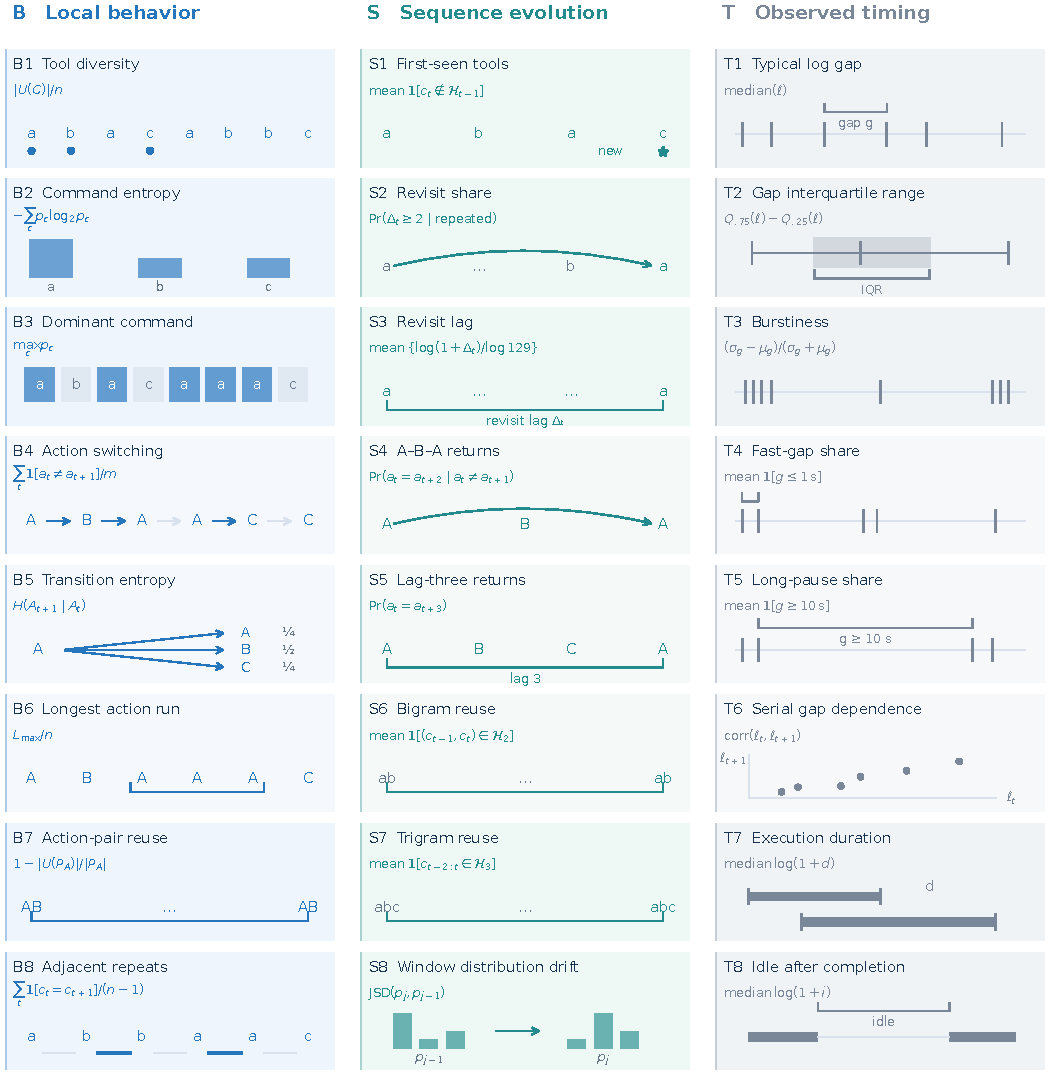
\includegraphics[width=.90\linewidth]{fingerprint-bst-dimensions.pdf}
\caption{The 24-slot B/S/T candidate schema, using the block colors of Figure~\ref{fig:architecture}. Glyphs illustrate definitions. Lowercase symbols denote commands and uppercase symbols coarse actions. $n$ counts window events, $m$ valid adjacent action pairs, $U$ unique values, $\mathcal{H}$ prefix history, and $\Delta_t$ revisit lag. For observed launch-gap timing, $g$ is a nonnegative gap in seconds and $\ell=\log(1+g)$; duration $d$ and post-duration idle $i$ are optional measurements not present in AIT.}
\label{fig:bst-dimensions}
\end{figure}

\FloatBarrier
\section{Evaluation}
\subsection{Datasets and observed fields}
Table~\ref{tab:cohorts} summarizes the three evaluation sources, their observed fields, and their roles in the study. Each relation label identifies a benchmark task within its source.

\begin{table}[ht]
\centering\compacttable
\caption{Evaluation cohorts and observation contracts. Counts describe the eligible trace views; unavailable timing is not inferred.}
\label{tab:cohorts}
\begin{tabularx}{\linewidth}{@{}p{.16\linewidth}p{.20\linewidth}p{.13\linewidth}p{.22\linewidth}Y@{}}
\toprule
Source & Records; tasks & Modes & Observed trace fields & Evaluation role \\
\midrule
CTH mixture core & 85 traces; 17 CTF tasks & \mixedmodes & Ordered commands; timing unavailable in normalized views; B/S & Five Agent shares and matched association \\
AIT audit logs & 109 runs; 12 tasks & \mixedmodes & Ordered commands; launch times; no durations; B/S + T1--T6 & Timing ablation and separate mode recognition \\
NYU D-CIPHER~\cite{nyu} & 585 runs; 160 challenges & \mbox{A\,\agenticon} & Ordered \texttt{run\_command} events; no timing; B/S & Frozen external Agent--Agent retrieval \\
\bottomrule
\end{tabularx}
\end{table}

The CTH timing entries above describe the normalized trace views used by this study, not every field in the upstream archive. The public archive also contains Human terminal I/O timing and timestamped Agent events, but their event units differ; we have not validated a common per-command start/end mapping and therefore do not use them as a matched timing cohort~\cite{cth,inspect}.

\FloatBarrier
\subsection{Pairing and validation}
\paragraph{Exact CTH role mixture.} The frozen CTH core has 17 task groups. In 170 coupled allocations, 16 tasks contribute query and candidate roles, with exactly 0, 8, 16, 24, or 32 Agent roles among the 32 allocated roles. Each query has one same-task and three different-task candidates. Candidate tasks and draws are paired across shares. The share is therefore a property of the constructed query galleries, not a resampled proportion of all source records. We retain the earlier command- and action-bigram-cosine baselines to describe this protocol.

\paragraph{Matched classifier and ablation tests.} The main CTH comparison uses the same 54,400 candidate-pair decisions for E and E+B/S across all five shares and all three learners. AIT contains 109 independent troubleshooting runs across 12 tasks; each configuration uses the same 43,600 pair decisions, with six observed launch-gap features (T1--T6) computed from recorded process timestamps. T7--T8 are all missing in this source. NYU contains 585 runs from four snapshots of one Agent framework, grouped into 160 challenge tasks not used in CTH development. Every NYU query is tested against one same-challenge and three different-challenge candidates. This is an AA-only cross-source test, and a challenge filename is the task-retrieval proxy.

The pipeline has two adaptive stages. Source fields determine which evidence blocks can be computed (AIT supplies launch gaps T1--T6; the normalized CTH and NYU views have no timing), while task-disjoint inner folds select preprocessing, window representation, fusion, classifier settings, and thresholds. For the CTH XGBoost B/S arm, all three outer folds select four-event windows; fold 0 selects mean/standard-deviation pooling with conditional fusion and depth 2, while folds 1 and 2 select mean/standard-deviation/trend pooling with direct fusion and depth 3. Each evidence arm selects its threshold on inner out-of-fold predictions under the FMR-at-most-10\% rule, then freezes it for the outer evaluation. This target is not expected to transfer to held-out tasks. CTH results average task outcomes and then the five shares equally; AIT and NYU average task outcomes. We use 10,000 paired task-cluster bootstrap resamples for intervals. Repeated gallery draws and pair decisions within a task are not independent observations, so intervals describe task-cluster uncertainty and remain approximate under shared candidates. No results are adjusted for the many development analyses.

We report balanced accuracy (BA), false-merge rate (FMR), and false-split rate (FSR), where $\mathrm{BA}=1-(\mathrm{FMR}+\mathrm{FSR})/2$. Increasing one error can therefore be hidden by a reduction in the other; all three measures are shown.

For threshold-free ranking, we calculate query-level Hit@1, Hit@2, MRR, and gallery AUC; the main comparison reports Hit@1, gallery AUC, and candidate-pair average precision (AP). Gallery AUC compares the one same-task candidate against the three different-task candidates for each query, assigning half credit to ties. Pair AP pools scores within each query task and role-share cell at the fixed one-to-three candidate ratio; CTH averages its five role shares equally within task. All intervals resample query-task clusters, so repeated galleries and pairs remain within their source task.

\section{Results}
\subsection{The mixture baseline shifts toward missed links}
Figure~\ref{fig:exact-mixture} shows both error rates and BA under the exact CTH role mixture. Command-cosine BA changes from 53.59\% at 0\% Agent roles to 46.50\% at 100\% (endpoint difference $-7.10\pp$, 95\% task interval $[-15.45,+0.06]$). Action-bigram BA changes from 57.40\% to 46.48\% ($-10.92\pp$, $[-20.61,-3.06]$). At the fixed threshold, missed links increase and false merges decrease from the first endpoint to the last.

\begin{figure}[!htbp]
\centering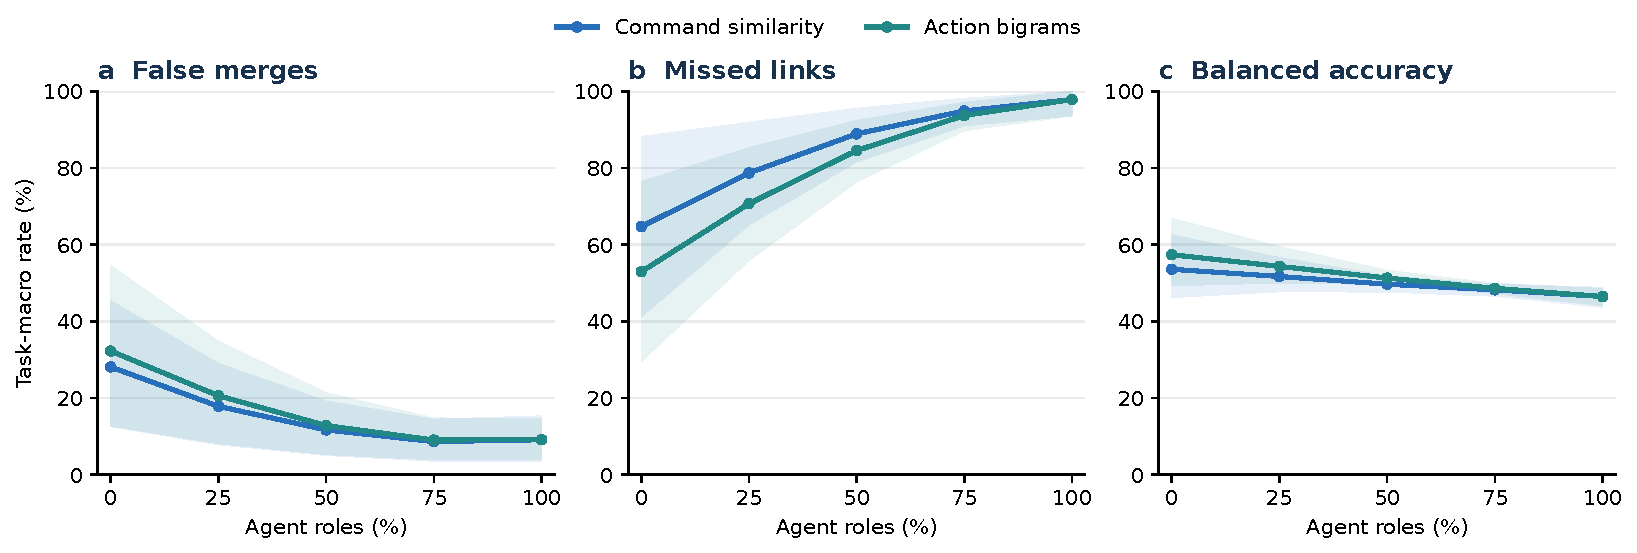
\includegraphics[width=\linewidth]{exact-mixture-v3.pdf}
\caption{Command and action-bigram cosine baselines at the five exact CTH role shares. From left to right, false merges, missed links, and balanced accuracy. Shading shows 95\% intervals from resampling the 17 task groups after averaging paired allocations within each task.}
\label{fig:exact-mixture}
\end{figure}

\subsection{Block effects depend on learner and target}
Figure~\ref{fig:cth-five-share} shows the matched E and E+B/S curves across the five shares. Table~\ref{tab:feature-block-ablation} completes the CTH single-block ablation and adds the full AIT block factorial on the same frozen candidate sets. The CTH results do not support one learner-independent B/S effect: SVM gains 1.51 BA points with B alone and 1.38 with B+S; the tree loses BA for every added block and its full B+S arm rejects every candidate; XGBoost is nearly unchanged with S alone (+0.04) but loses 3.31 points with B alone and 2.38 with B+S. Thus the block choice changes which errors are exchanged, and the selected classifier matters. All CTH BA intervals include zero, although some changes in the component error rates do not; the experiment record preserves paired intervals and fold-level details. Figure~\ref{fig:cth-delta} retains the share-specific comparison for the full B/S arm.

\begin{figure}[ht]
\centering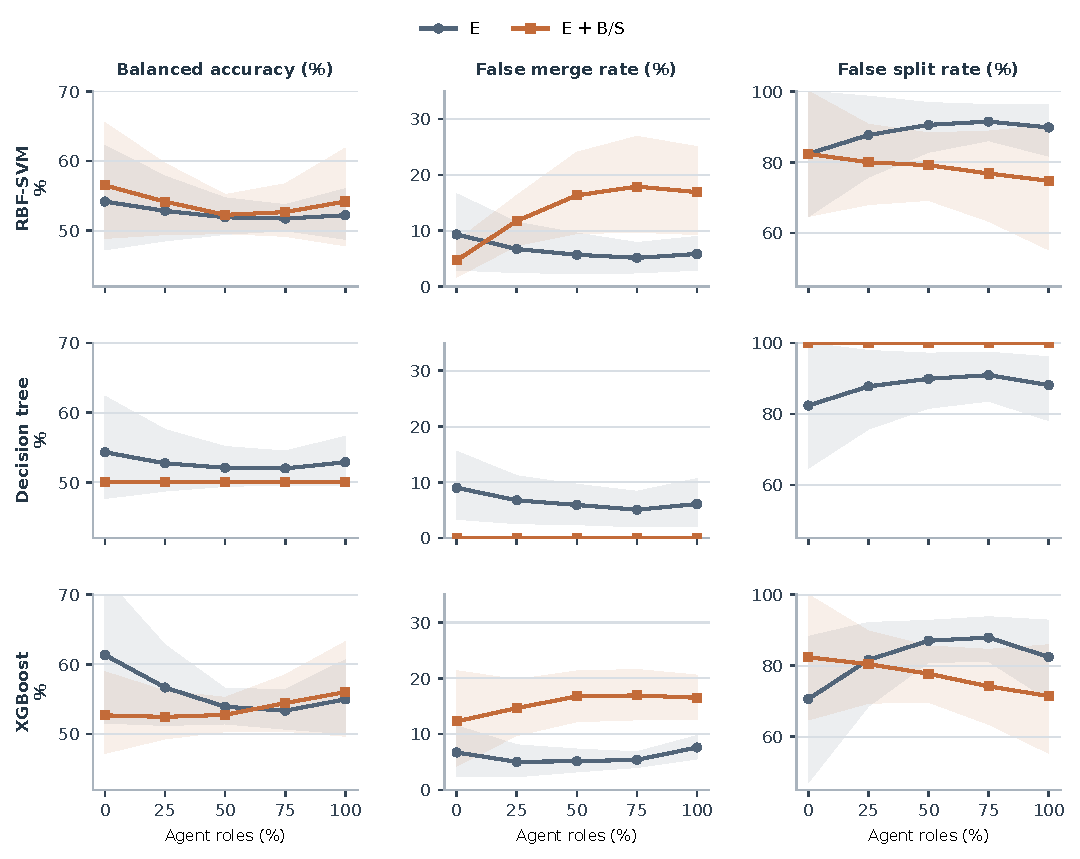
\includegraphics[width=\linewidth]{cth-five-share-matched.pdf}
\caption{Matched CTH comparison over exact Agent-role shares. Rows are learners; columns are BA, FMR, and FSR. Lines show E and E+B/S, and bands show 95\% task-cluster intervals. Y-ranges are shared within each metric column and stated by the axes. The role percentage is over query and candidate roles.}
\label{fig:cth-five-share}
\end{figure}

\begin{figure}[!b]
\centering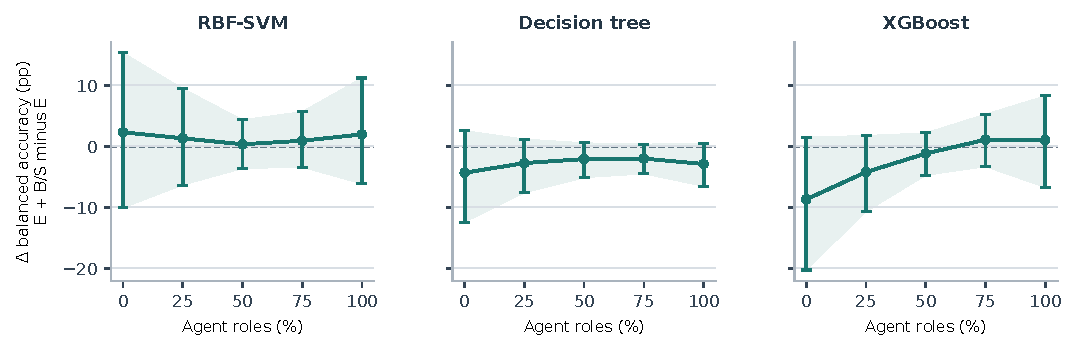
\includegraphics[width=.92\linewidth]{cth-five-share-delta-ba.pdf}
\caption{Paired BA change (E+B/S minus E) at each CTH share, in percentage points. The dashed line marks zero; intervals are task-cluster paired 95\% intervals.}
\label{fig:cth-delta}
\end{figure}

\begin{table}[ht]
\centering
\scriptsize\setlength{\tabcolsep}{3pt}\renewcommand{\arraystretch}{1.1}
\caption{Matched CTH classifier comparison averaged equally over five Agent-role shares. Every classifier uses the same paired candidate decisions. Changes are B/S minus evidence-only E in percentage points; 95\% intervals are paired task-cluster bootstrap intervals.}
\label{tab:cth-matched-classifiers}
\begin{tabular*}{\linewidth}{@{\extracolsep{\fill}}lrrrrr@{}}
\toprule
Classifier & BA: E & BA: E+B/S & $\Delta$BA [95\% CI] & $\Delta$FMR & $\Delta$FSR \\ \midrule
RBF-SVM & 52.57 & 53.95 & $+1.38\;[-3.83,+6.53]$ & +6.99 & -9.74 \\
Decision tree & 52.80 & 50.00 & $-2.80\;[-6.61,+0.57]$ & -6.59 & +12.19 \\
XGBoost & 56.06 & 53.68 & $-2.38\;[-7.13,+2.25]$ & +9.46 & -4.70 \\
\bottomrule
\end{tabular*}
\end{table}


As a separate post-hoc diagnostic, XGBoost gains a conditional signal when training pairs are expanded and E includes value-redacted argument syntax. On the same 17 CTH tasks, E+Args+B/S versus E+Args changes BA by $+6.25\pp$ (nominal 95\% task interval $[+1.17,+12.24]$), FSR by $-13.06\pp$, and FMR by $+0.56\pp$. The max-T interval across four related contrasts includes zero ($[-0.75,+13.24]$); this exploratory result does not overturn the primary matched comparison.

\subsection{Pair type changes the error pattern, not the conclusion}
We reuse the same XGBoost predictions and average only the shares where each candidate-pair type exists. For HH, the BA difference is $-8.84\pp$ $[-20.34,+1.67]$; HA is $+1.29\pp$ $[-1.78,+4.71]$; AA is $+1.39\pp$ $[-5.80,+8.03]$. HA and AA point gains accompany higher FMR, while HH trends downward in BA. No stratum establishes a reliable gain. Pair types describe the modes assigned to the two traces and say nothing about whether their behaviors came from the same real attack or operator (Appendix~\ref{app:pair-types}).

\subsection{AIT timing and external Agent-only transfer}
On AIT, all feature arms have positive BA point changes relative to E, but their ranking point estimates are lower than E. The isolated T1--T6 increment over E+B/S is +0.98 BA points; the paired task interval includes zero. Hit@1, gallery AUC, and pair AP also have positive but uncertain increments. This comparison does not evaluate duration or post-completion idle time (T7--T8), which are unobserved. AIT task and collection workflow covary with recorded role, so these timing results remain specific to this troubleshooting cohort.

On frozen NYU Agent-only retrieval, XGBoost gains 5.71 BA points but its FMR reaches 25.39\% despite the 10\% CTH calibration target; the decision tree's BA gain comes with lower ranking scores, while SVM loses 8.23 BA points. Table~\ref{tab:ranking-diagnostics} shows absolute ranking values and paired changes together. It makes clear that thresholded BA and candidate ordering can move in opposite directions.

\begin{table}[!htbp]
\centering
\small
\setlength{\tabcolsep}{3.5pt}
\renewcommand{\arraystretch}{1.10}
\caption{Candidate-ranking performance for the predeclared feature comparisons.}
\label{tab:ranking-diagnostics}
\begin{tabularx}{\linewidth}{@{}p{1.02in}Yrrr@{}}
\toprule
Learner & Scored evidence & Hit@1 (\%) & Gallery AUC (\%) & Pair AP (\%) \\
\midrule
\multicolumn{5}{@{}l}{\textbf{CTH mixed roles: E+B+S compared with E}} \\
\textbf{RBF-SVM} & \textbf{E (baseline)} & \textbf{33.75} & \textbf{58.73} & \textbf{39.78} \\
 & \quad E+B+S & \cellcolor{AblGoodMid}38.45{\scriptsize\,(+4.70)} & \cellcolor{AblGoodMid}62.22{\scriptsize\,(+3.49)} & \cellcolor{AblGoodLight}42.66{\scriptsize\,(+2.88)} \\
\addlinespace[.15em]
\textbf{Decision tree} & \textbf{E (baseline)} & \textbf{34.91} & \textbf{60.30} & \textbf{35.21} \\
 & \quad E+B+S & \cellcolor{AblGoodLight}36.27{\scriptsize\,(+1.37)} & 59.77{\scriptsize\,(-0.53)} & \cellcolor{AblGoodLight}36.44{\scriptsize\,(+1.23)} \\
\addlinespace[.15em]
\textbf{XGBoost} & \textbf{E (baseline)} & \textbf{34.40} & \textbf{58.92} & \textbf{40.97} \\
 & \quad E+B+S & \cellcolor{AblGoodLight}37.01{\scriptsize\,(+2.61)} & \cellcolor{AblGoodLight}61.73{\scriptsize\,(+2.81)} & 41.06{\scriptsize\,(+0.08)} \\
\midrule
\multicolumn{5}{@{}l}{\textbf{AIT XGBoost: T increment is compared with E+B+S}} \\
\textbf{XGBoost} & \textbf{E (baseline)} & \textbf{40.20} & \textbf{63.34} & \textbf{38.25} \\
 & \quad E+B+S & \cellcolor{AblBadMid}33.33{\scriptsize\,(-6.88)} & \cellcolor{AblBadMid}57.87{\scriptsize\,(-5.47)} & \cellcolor{AblBadMid}32.60{\scriptsize\,(-5.65)} \\
 & \quad E+B+S+T1--T6$^{\dagger}$ & 34.01{\scriptsize\,(+0.68)} & 58.80{\scriptsize\,(+0.93)} & \cellcolor{AblGoodLight}34.11{\scriptsize\,(+1.50)} \\
\midrule
\multicolumn{5}{@{}l}{\textbf{NYU Agent-only external evaluation: frozen E+B+S compared with E}} \\
\textbf{RBF-SVM} & \textbf{E (baseline)} & \textbf{39.73} & \textbf{65.75} & \textbf{42.77} \\
 & \quad E+B+S & \cellcolor{AblBadLight}38.67{\scriptsize\,(-1.06)} & 65.56{\scriptsize\,(-0.18)} & \cellcolor{AblBadLight}41.35{\scriptsize\,(-1.41)} \\
\addlinespace[.15em]
\textbf{Decision tree} & \textbf{E (baseline)} & \textbf{36.92} & \textbf{63.94} & \textbf{35.29} \\
 & \quad E+B+S & \cellcolor{AblBadMid}31.33{\scriptsize\,(-5.59)} & \cellcolor{AblBadMid}56.80{\scriptsize\,(-7.13)} & \cellcolor{AblBadLight}32.29{\scriptsize\,(-3.00)} \\
\addlinespace[.15em]
\textbf{XGBoost} & \textbf{E (baseline)} & \textbf{34.74} & \textbf{61.29} & \textbf{39.55} \\
 & \quad E+B+S & \cellcolor{AblGoodMid}37.94{\scriptsize\,(+3.20)} & \cellcolor{AblGoodLight}63.10{\scriptsize\,(+1.82)} & \cellcolor{AblGoodLight}41.62{\scriptsize\,(+2.07)} \\
\bottomrule
\end{tabularx}
\par\vspace{.16em}
\begin{minipage}{\linewidth}\footnotesize
Cells give absolute task-macro percentages and signed paired changes in parentheses. CTH and NYU changes compare E+B+S with E; the AIT $\dagger$ row gives the incremental change over E+B+S. Higher ranking values are favorable. Pale-to-deeper teal/red backgrounds encode fixed absolute-change bands of 1--$<3$, 3--$<8$, and $\geq8$ points; changes below 1 point are unshaded. Colors do not encode statistical significance. If any pair in a four-candidate gallery lacks a required block, all four ranking scores use the matched E score. Complete factorial ranking estimates are in the appendix; task-cluster intervals are in the experiment record.
\end{minipage}
\end{table}


\FloatBarrier
\section{Discussion}
The clearest result is a change in the fixed-threshold operating point as CTH gallery composition changes. From all-Human to all-Agent allocations, the action-bigram baseline's FMR falls by $23.09\pp$ while its FSR rises by $44.93\pp$. Hit@1 is nearly unchanged ($-0.05\pp$, 95\% interval $[-12.96,+12.91]$), and gallery AUC declines by $11.48\pp$ with an interval spanning zero. The error shift therefore does not show that Agent-heavy galleries rank candidates better; it shows why a thresholded link decision and a ranking score answer different questions.

The primary matched CTH comparison finds no common B/S gain across learners. The post-hoc XGBoost result is conditional on expanded training-pair support and redacted argument syntax; its multiplicity-adjusted interval includes zero. NYU shows that the signal can transfer differently by learner: XGBoost improves Hit@1 and pair AP, but its B/S FMR reaches 25.39\% despite the 10\% CTH validation target; the decision tree's BA gain comes with worse ranking. AIT's observed launch-gap increment is uncertain. These findings do not isolate whether pair differences arise from execution behavior, capture interface, trace volume, or threshold transfer.

The association label is benchmark-task identity, not a shared-activity or actor label. CTH records Human terminal input and Agent tool calls through different interfaces; pair-type estimates reuse overlapping tasks and are descriptive. In the separate NYU snapshot test, B/S adds a small ranking increment with full traces, while fixed-prefix estimates are uncertain (Appendix~\ref{app:snapshot-retrieval}). Repeated galleries share tasks and candidates, so task-cluster intervals remain approximate.

\section{Conclusion}
Taken together, we propose a general, observation-aware framework for Agent-aware trace association. It augments command evidence with explicit local-behavior (B), sequence (S), and timing (T) dimensions when a source provides them, while keeping Human/Agent mode estimation as a separate readout. These named measurements provide an interpretable basis for characterizing recorded execution mode and examining how behavior, sequence, and time contribute to candidate links. The fold-adaptive pipeline selects usable evidence blocks, window summaries, fusion, learner, and threshold within task-disjoint training folds, then freezes those choices for held-out evaluation. In our measurements, gallery composition shifts a fixed threshold from false merges toward missed links; B/S gains depend on the learner, source, and training setup, while the AIT timing increment remains uncertain. This gives researchers a reusable method for integrating Agent-related dimensions and testing whether they improve retrieval, with current benchmarks showing conditional utility rather than a universal performance guarantee. Same-challenge labels remain retrieval proxies and do not establish shared attack activity or operator identity.

\begin{thebibliography}{99}
\bibitem{syntheticapt} F. Balassone et al. ``Synthetic APTs: the Collapse of TTP-Based Attribution.'' arXiv:2606.07158, 2026. \url{https://arxiv.org/abs/2606.07158}
\bibitem{trace} Murali Ediga and Sudipta Chattopadhyay. ``Trace: Unmasking AI Attack Agents Through Terminal Behavior Fingerprinting.'' arXiv:2605.01186, 2026. \url{https://arxiv.org/abs/2605.01186}
\bibitem{procgrep} Hamidah Oderinwale. ``Agent Trajectories as Programs: Fingerprinting and Programming Coding-Agent Behavior.'' arXiv:2606.16988, 2026. \url{https://arxiv.org/abs/2606.16988}
\bibitem{lidar} Chuyi Wang et al. ``Who Is Behind the Harness? Fingerprinting LLMs through Agentic Behavior.'' arXiv:2609.28559, 2026. \url{https://arxiv.org/abs/2609.28559}
\bibitem{known} William Lugoloobi et al. ``Known By Their Actions: Fingerprinting LLM Browser Agents via UI Traces.'' arXiv:2605.14786, 2026. \url{https://arxiv.org/abs/2605.14786}
\bibitem{cybias} Taein Lim et al. ``CyBiasBench: Benchmarking Bias in LLM Agents for Cyber-Attack Scenarios.'' arXiv:2605.07830, 2026. \url{https://arxiv.org/abs/2605.07830}
\bibitem{crossagent} SangJin Park et al. ``Cross-Agent Campaign Attribution: Linking Asynchronous Attacks Across LLM Agents.'' arXiv:2607.18826, 2026. \url{https://arxiv.org/abs/2607.18826}
\bibitem{honey} ``Honey for the Agent: Cyber Deception and Behavioral Fingerprinting.'' Zenodo record 20818246, 2026. \url{https://zenodo.org/records/20818246}
\bibitem{cth} Lyptus Research. ``Cyber Task Horizons Data.'' 2026. \url{https://github.com/lyptus-research/cyber-task-horizons-data}
\bibitem{mcmahon} M. M. McMahon and H. A. Sholl. ``Influence of State Size on User Models in a Network Security System.'' 13th International Conference on Parallel and Distributed Computing Systems, 2000. \url{https://www.researchgate.net/publication/282647993_Influence_of_State_Size_on_User_Models_in_a_Network_Security_System}
\bibitem{dao} V. N. P. Dao, R. Vemuri, and S. J. Templeton. ``Profiling Users in the UNIX OS Environment.'' Lawrence Livermore National Laboratory preprint UCRL-JC-141022, 2000. \url{https://www.osti.gov/servlets/purl/15004770}
\bibitem{inspect} UK AI Safety Institute. ``Inspect AI: Event Reference.'' \url{https://inspect.aisi.org.uk/reference/inspect_ai.event.html}
\bibitem{atlas} A. Alsaheel et al. ``ATLAS: A Sequence-Based Learning Approach for Attack Investigation.'' USENIX Security Symposium, 2021. \url{https://www.usenix.org/conference/usenixsecurity21/presentation/alsaheel}
\bibitem{holmes} M. Milajerdi et al. ``HOLMES: Real-Time APT Detection through Correlation of Suspicious Information Flows.'' IEEE Symposium on Security and Privacy, 2019. \url{https://arxiv.org/abs/1810.01594}
\bibitem{ostinato} Sutanu Kumar Ghosh et al. ``OSTINATO: Cross-Host Attack Correlation through Attack Activity Similarity Detection.'' arXiv:2312.09321, 2023. \url{https://arxiv.org/abs/2312.09321}
\bibitem{poirot} Sadegh M. Milajerdi et al. ``POIROT: Aligning Attack Behavior with Kernel Audit Records for Cyber Threat Hunting.'' CCS, 2019. \url{https://arxiv.org/abs/1910.00056}
\bibitem{sfm} Yi-Ting Huang et al. ``A Cascade Approach for APT Campaign Attribution in System Event Logs: Technique Hunting and Subgraph Matching.'' arXiv:2410.22602, 2024. \url{https://arxiv.org/abs/2410.22602}
\bibitem{intercode} H. Yang et al. ``InterCode: Standardizing and Benchmarking Interactive Coding with Execution Feedback.'' NeurIPS, 2023. \url{https://arxiv.org/abs/2306.14898}
\bibitem{nyu} NYU-LLM-CTF. ``Leaderboard Submissions.'' GitHub repository, revision recorded in the frozen evaluation manifest. \url{https://github.com/NYU-LLM-CTF/leaderboard_submissions}
\end{thebibliography}

\appendix
\section{Supplementary CTH and external results}
Figure~\ref{fig:cth-pair-type} displays paired changes by role type, while Table~\ref{tab:cth-per-share-xgb} gives exact XGBoost values by mixture share. The external table reports learner-specific absolute results and the paired error changes; its intervals cluster the 160 held-out challenge groups.

\begin{figure}[ht]
\centering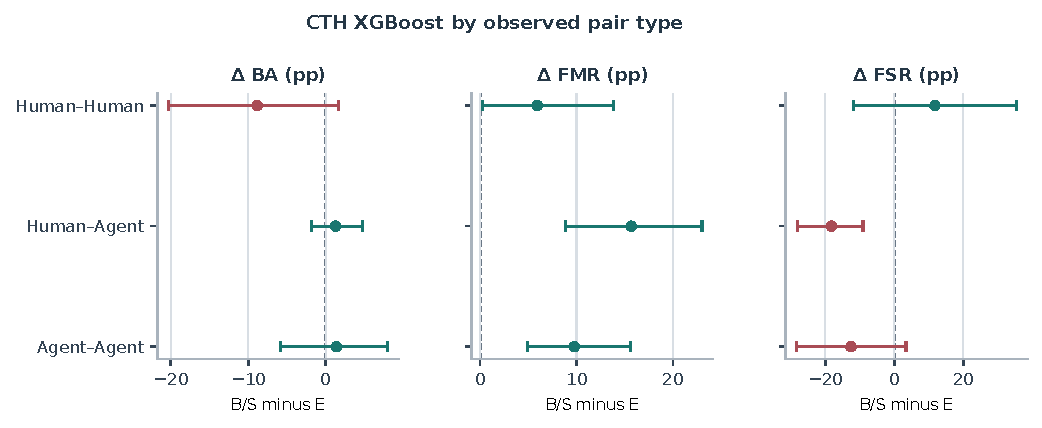
\includegraphics[width=.95\linewidth]{cth-xgb-pair-type-deltas.pdf}
\caption{CTH XGBoost change (E+B/S minus E) by pair type and metric. Points are share-equal means over the eligible proportions; bars show paired task-cluster 95\% intervals. HH, HA, and AA are evaluation roles, not attack identities.}
\label{fig:cth-pair-type}
\end{figure}
\begin{table}[ht]
\centering
\scriptsize\setlength{\tabcolsep}{2.5pt}\renewcommand{\arraystretch}{1.1}
\caption{Frozen NYU D-CIPHER AA challenge-retrieval comparison. The challenge filename defines the same-task proxy. Changes are E+B/S minus E; intervals cluster by 160 task groups.}
\label{tab:nyu-aa-confirmation}
\begin{tabular*}{\linewidth}{@{\extracolsep{\fill}}lrrrrrr@{}}
\toprule
Classifier & BA: E & BA: E+B/S & $\Delta$BA [95\% CI] & FMR: E+B/S & $\Delta$FMR & $\Delta$FSR \\ \midrule
RBF-SVM & 58.16 & 49.93 & $-8.23\;[-10.22,-6.28]$ & 0.13 & -26.45 & +42.91 \\
Decision tree & 49.69 & 53.33 & $+3.64\;[+1.97,+5.37]$ & 8.54 & +4.69 & -11.98 \\
XGBoost & 51.16 & 56.87 & $+5.71\;[+3.63,+7.73]$ & 25.39 & +14.67 & -26.10 \\
\bottomrule
\end{tabular*}
\end{table}

\begin{table}[ht]
\centering
\scriptsize\setlength{\tabcolsep}{3pt}\renewcommand{\arraystretch}{1.1}
\caption{CTH XGBoost error changes by pair type, averaged equally over the role shares where the type exists. HH, HA, and AA are trace-role pairs, not activity or actor labels.}
\label{tab:cth-pair-type-deltas}
\begin{tabular*}{\linewidth}{@{\extracolsep{\fill}}lrrr@{}}
\toprule
Pair type & $\Delta$BA [95\% CI] & $\Delta$FMR & $\Delta$FSR \\ \midrule
Human--Human & $-8.84\;[-20.34,+1.67]$ & +5.92 & +11.76 \\
Human--Agent & $+1.29\;[-1.78,+4.71]$ & +15.66 & -18.23 \\
Agent--Agent & $+1.39\;[-5.80,+8.03]$ & +9.77 & -12.54 \\
\bottomrule
\end{tabular*}
\end{table}

\begin{table}[ht]
\centering
\scriptsize\setlength{\tabcolsep}{2.6pt}\renewcommand{\arraystretch}{1.08}
\caption{CTH XGBoost results by exact Agent-role share. Values are task-macro means over the same paired candidates; $\Delta$BA intervals preserve task clustering.}
\label{tab:cth-per-share-xgb}
\begin{tabular*}{\linewidth}{@{\extracolsep{\fill}}rrrrrr@{}}
\toprule
Agent roles & BA: E & BA: E+B/S & $\Delta$BA [95\% CI] & FMR: E+B/S & FSR: E+B/S \\ \midrule
0\% & 61.35 & 52.68 & $-8.67\;[-20.26,+1.53]$ & 12.28 & 82.35 \\
25\% & 56.68 & 52.47 & $-4.21\;[-10.70,+1.79]$ & 14.66 & 80.40 \\
50\% & 53.92 & 52.76 & $-1.16\;[-4.74,+2.22]$ & 16.76 & 77.72 \\
75\% & 53.36 & 54.45 & $+1.10\;[-3.33,+5.29]$ & 16.94 & 74.15 \\
100\% & 54.99 & 56.03 & $+1.04\;[-6.73,+8.28]$ & 16.51 & 71.43 \\
\bottomrule
\end{tabular*}
\end{table}


\subsection{Complete factorial ranking ablation}
The main ranking table shows the predeclared contrasts; Table~\ref{tab:full-ranking-ablation} preserves every CTH and AIT feature combination. For ranking, any gallery with at least one unavailable pairwise block is scored entirely with its matched E baseline so all four candidates share one scoring scale.
\begin{table}[!htbp]
\centering
\scriptsize
\setlength{\tabcolsep}{3pt}
\renewcommand{\arraystretch}{1.07}
\caption{Complete factorial ranking ablation. Values are absolute percentages followed by changes from E.}
\label{tab:full-ranking-ablation}
\begin{tabularx}{\linewidth}{@{}p{.82in}p{1.15in}Yrrr@{}}
\toprule Source & Learner & Feature arm & Hit@1 & Gallery AUC & Pair AP \\
\midrule
CTH & \textbf{RBF-SVM} & \textbf{E (baseline)} & \textbf{33.75} & \textbf{58.73} & \textbf{39.78} \\
 &  & \quad E+B & \cellcolor{AblGoodMid}36.93{\scriptsize\,(+3.18)} & \cellcolor{AblGoodLight}60.63{\scriptsize\,(+1.90)} & \cellcolor{AblGoodLight}40.90{\scriptsize\,(+1.13)} \\
 &  & \quad E+S & \cellcolor{AblGoodLight}35.52{\scriptsize\,(+1.77)} & \cellcolor{AblGoodLight}61.67{\scriptsize\,(+2.94)} & 40.57{\scriptsize\,(+0.79)} \\
 &  & \quad E+B+S & \cellcolor{AblGoodMid}38.45{\scriptsize\,(+4.70)} & \cellcolor{AblGoodMid}62.22{\scriptsize\,(+3.49)} & \cellcolor{AblGoodLight}42.66{\scriptsize\,(+2.88)} \\
\addlinespace[.12em]
 & \textbf{Decision tree} & \textbf{E (baseline)} & \textbf{34.91} & \textbf{60.30} & \textbf{35.21} \\
 &  & \quad E+B & \cellcolor{AblBadMid}27.49{\scriptsize\,(-7.41)} & \cellcolor{AblBadMid}53.62{\scriptsize\,(-6.69)} & \cellcolor{AblBadMid}30.90{\scriptsize\,(-4.31)} \\
 &  & \quad E+S & \cellcolor{AblBadLight}32.08{\scriptsize\,(-2.83)} & \cellcolor{AblBadMid}56.14{\scriptsize\,(-4.17)} & \cellcolor{AblBadLight}34.07{\scriptsize\,(-1.15)} \\
 &  & \quad E+B+S & \cellcolor{AblGoodLight}36.27{\scriptsize\,(+1.37)} & 59.77{\scriptsize\,(-0.53)} & \cellcolor{AblGoodLight}36.44{\scriptsize\,(+1.23)} \\
\addlinespace[.12em]
 & \textbf{XGBoost} & \textbf{E (baseline)} & \textbf{34.40} & \textbf{58.92} & \textbf{40.97} \\
 &  & \quad E+B & 33.53{\scriptsize\,(-0.87)} & 58.81{\scriptsize\,(-0.11)} & \cellcolor{AblBadLight}38.98{\scriptsize\,(-1.99)} \\
 &  & \quad E+S & \cellcolor{AblGoodLight}36.95{\scriptsize\,(+2.55)} & \cellcolor{AblGoodLight}61.49{\scriptsize\,(+2.57)} & 40.68{\scriptsize\,(-0.30)} \\
 &  & \quad E+B+S & \cellcolor{AblGoodLight}37.01{\scriptsize\,(+2.61)} & \cellcolor{AblGoodLight}61.73{\scriptsize\,(+2.81)} & 41.06{\scriptsize\,(+0.08)} \\
\addlinespace[.12em]
\midrule
AIT & \textbf{XGBoost} & \textbf{E (baseline)} & \textbf{40.20} & \textbf{63.34} & \textbf{38.25} \\
 &  & \quad E+B & \cellcolor{AblBadMid}34.20{\scriptsize\,(-6.00)} & \cellcolor{AblBadMid}57.47{\scriptsize\,(-5.86)} & \cellcolor{AblBadMid}33.35{\scriptsize\,(-4.90)} \\
 &  & \quad E+S & \cellcolor{AblBadMid}37.05{\scriptsize\,(-3.15)} & \cellcolor{AblBadMid}60.31{\scriptsize\,(-3.02)} & \cellcolor{AblBadLight}35.80{\scriptsize\,(-2.45)} \\
 &  & \quad E+T1--T6 & \cellcolor{AblBadLight}39.02{\scriptsize\,(-1.19)} & 62.78{\scriptsize\,(-0.56)} & \cellcolor{AblBadLight}36.73{\scriptsize\,(-1.52)} \\
 &  & \quad E+B+S & \cellcolor{AblBadMid}33.33{\scriptsize\,(-6.88)} & \cellcolor{AblBadMid}57.87{\scriptsize\,(-5.47)} & \cellcolor{AblBadMid}32.60{\scriptsize\,(-5.65)} \\
 &  & \quad E+B+T1--T6 & \cellcolor{AblBadMid}35.53{\scriptsize\,(-4.67)} & \cellcolor{AblBadMid}59.46{\scriptsize\,(-3.88)} & \cellcolor{AblBadMid}33.96{\scriptsize\,(-4.29)} \\
 &  & \quad E+S+T1--T6 & \cellcolor{AblBadLight}38.02{\scriptsize\,(-2.18)} & \cellcolor{AblBadLight}61.70{\scriptsize\,(-1.64)} & \cellcolor{AblBadLight}36.76{\scriptsize\,(-1.49)} \\
 &  & \quad E+B+S+T1--T6 & \cellcolor{AblBadMid}34.01{\scriptsize\,(-6.19)} & \cellcolor{AblBadMid}58.80{\scriptsize\,(-4.53)} & \cellcolor{AblBadMid}34.11{\scriptsize\,(-4.14)} \\
\addlinespace[.12em]
\bottomrule
\end{tabularx}
\par\vspace{.12em}
\begin{minipage}{\linewidth}\footnotesize
Each change is a paired task-level percentage-point difference from the same learner/source E baseline; the AIT $+$T increment is separately shown in the main ranking table. Teal/red shading uses the fixed magnitude bands described in Table~\ref{tab:ranking-diagnostics}; colors do not encode significance. CTH includes 17 task clusters and 54,400 pair decisions per arm; AIT includes 12 clusters and 43,600 decisions per arm. Gallery ranking uses whole-gallery E fallback when any candidate lacks a required block. Intervals, tie counts, and fallback details are recorded in the accompanying experiment Markdown and JSON.
\end{minipage}
\end{table}


\begin{figure}[ht]
\centering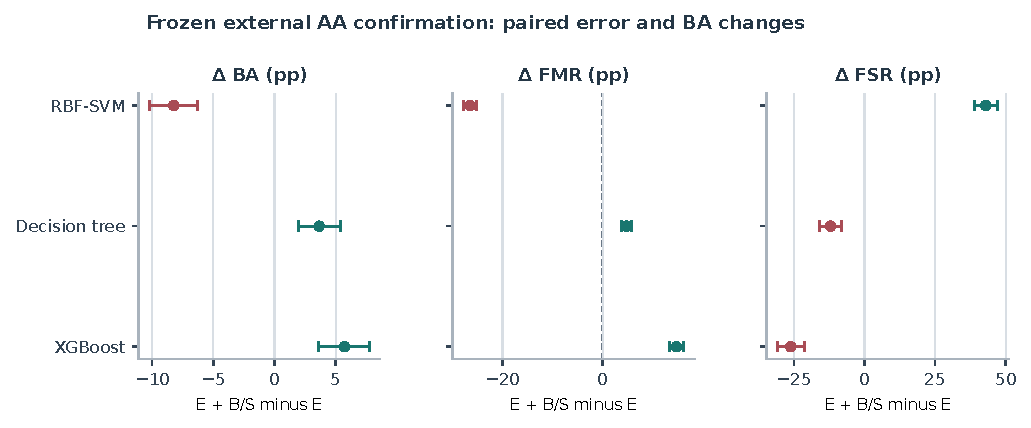
\includegraphics[width=.95\linewidth]{nyu-aa-paired-deltas.pdf}
\caption{Frozen NYU AA evaluation: paired changes in BA, FMR, and FSR for E+B/S relative to E. The vertical dashed reference is zero; intervals cluster 160 challenge groups.}
\label{fig:nyu-deltas}
\end{figure}

\section{Frozen external evaluation protocol}\label{app:nyu}
The NYU task manifest was frozen before fitting. Four public D-CIPHER snapshots from the official NYU-LLM-CTF leaderboard-submissions repository were included~\cite{nyu}. The exact source revision and hashes are in the frozen evaluation manifest. Challenge groups overlapping the CTH development pool and one duplicate command sequence were removed. The remaining 160 groups and 585 runs were partitioned by a fixed hash into three retrieval galleries. For each run query, 100 deterministic draws selected one other run from the same challenge and one run from each of three different challenges in the same partition. All three classifiers and both feature arms used the identical 234,000-pair list. Training used only the 17 CTH development task groups and all available training pairs; model parameters and thresholds were not selected from NYU outcomes. The CTH-derived threshold did not preserve its target FMR on the external source.

\paragraph{Snapshot composition.} The evaluation contains four submissions of the same D-CIPHER framework. Table~\ref{tab:nyu-composition} reports how the raw transcripts map to eligible traces and distinct challenge groups. Challenge counts overlap across snapshots; the total is deduplicated.

\begin{table}[ht]
\centering\compacttable
\caption{NYU D-CIPHER snapshot composition. Challenge counts overlap across snapshots; the total counts distinct eligible challenges.}
\label{tab:nyu-composition}
\begin{tabularx}{\linewidth}{@{}Yrrr@{}}
\toprule
Model snapshot & Raw transcripts & Eligible traces & Eligible challenges \\
\midrule
Claude 3.5 Sonnet & 194 & \agentcount{147} & 147 \\
Claude 3.7 Sonnet & 200 & \agentcount{128} & 128 \\
GPT-4.1 & 196 & \agentcount{153} & 153 \\
GPT-4o & 197 & \agentcount{157} & 157 \\
\midrule
\textbf{Total} & 787 & \agentcount{585} & 160 \\
\bottomrule
\end{tabularx}
\end{table}

The official repository and snapshot metadata identify challenge filenames and run configuration. A shared challenge name is only the relation proxy. The four snapshots all belong to one Agent framework; this dataset cannot test Human--Agent associations or activity/actor attribution. Error transitions are counts of repeated pair decisions, not independent events: XGBoost corrected 11,241 earlier false merges and introduced 37,348 new false merges, while it corrected 19,708 earlier false splits and introduced 4,329 new false splits. These counts explain the rate changes but do not increase the independent sample size.

\section{Pair-type support and interpretation}\label{app:pair-types}
The CTH type-specific estimates reuse the outer predictions. HH is supported at 0--75\% Agent roles, HA at 25--75\%, and AA at 25--100\%. Each type is averaged equally across the shares where it exists and then across tasks. At 50\%, the XGBoost gallery contributes 662 positive and 2,004 negative HH pair decisions, 1,396 positive and 4,161 negative HA decisions, and 662 positive and 1,995 negative AA decisions. Pair decisions share queries, candidate tasks, and task clusters; the counts are denominators, not independent sample sizes. The interval widths and overlapping task support preclude interpreting the three rows as independent replications.

\FloatBarrier
\section{Fingerprint definitions and supplementary evaluations}\label{app:overnight-figures}
Table~\ref{tab:features} lists the feature definitions in Figure~\ref{fig:bst-dimensions}. The supplementary evaluations examine feature reduction, ranking loss, cross-challenge snapshot retrieval, and observed timing in AIT.

\begingroup\compacttable
\begin{longtable}{@{}p{0.08\linewidth}p{0.22\linewidth}p{0.62\linewidth}@{}}
\caption{Window-level feature definitions. A value is missing when its required observations are absent or insufficient.}\label{tab:features}\\
\toprule Block & ID & Measurement \\
\midrule\endfirsthead
\toprule Block & ID & Measurement \\
\midrule\endhead
B & B1--B3 & Distinct command share; Shannon entropy of command names; share of the dominant command. \\
B & B4--B6 & Fraction of known adjacent action pairs that switch group; conditional entropy of the next action; longest single-action run divided by window length. \\
B & B7--B8 & One minus the unique mapped adjacent-action-pair share; fraction of adjacent command names that are identical. \\
S & S1--S3 & First-seen command share; fraction of repeated commands whose previous occurrence is at least two positions back; mean normalized log revisit span. \\
S & S4--S5 & A-B-A action return share among valid triplets; share of valid four-action segments whose first and fourth action match. \\
S & S6--S8 & Reused adjacent command-bigram share; reused command-trigram share; Jensen--Shannon divergence between current and preceding window action distributions. \\
T & T1--T3 & Median log(1+gap); interquartile range of log gaps; burstiness $(\sigma-\mu)/(\sigma+\mu)$ over nonnegative raw gaps. \\
T & T4--T6 & Fraction of gaps at most one second; fraction at least ten seconds; lag-one correlation of log gaps when at least three valid gaps exist. \\
T & T7--T8 & Optional duration-dependent extensions: median log(1+observed event duration); median log(1+idle interval) after subtracting observed duration from the next start time. Not observed in AIT. \\
\bottomrule
\end{longtable}
\endgroup

\subsection{Exploratory single-measure reduction}
A nested diagnostic on the 17 CTH development tasks compared full B/S with 16 candidates, each dropping one window measurement. Inner task folds selected the deletion under the existing FMR-at-most-10\% threshold rule. The selected removals differed across folds (B6, S7, and B2). Both ranking and decision metrics use the E score on pairs with a missing block. Against full B/S, the compact version changed BA by $-0.59\pp$ (95\% task interval $[-2.02,+0.71]$), Hit@1 by $-0.24\pp$ $[-3.13,+2.15]$, gallery AUC by $-0.32\pp$ $[-1.92,+1.03]$, and pair AP by $-0.14\pp$ $[-1.75,+1.38]$. The results leave the value of deleting an individual measure uncertain.

\subsection{CTH ranking loss}
On the same 54,400 candidate pairs, we compared a logistic pair classifier with a logistic ranker trained on feature differences between positives and negatives for the same query. Both used identical training pairs and task weights. The inner folds selected regularization by gallery AUC and calibrated thresholds under the existing FMR rule. With E alone, changing the loss changed gallery AUC by $-0.49\pp$ $[-1.11,+0.02]$. With E+B/S, it changed AUC by $-5.90\pp$ $[-12.27,-1.06]$ and Hit@1 by $-6.97\pp$ $[-12.71,-2.17]$. The lowest held-out FMR among these four logistic arms was 13.83\%, above the 10\% validation target.

\subsection{Cross-challenge snapshot retrieval}\label{app:snapshot-retrieval}
This separate evaluation uses 111 NYU challenges with one trace from each of four D-CIPHER submissions (444 traces). Each query is matched against four runs from one different challenge, one per snapshot. Only the matching snapshot is positive. We hold out entire challenges, train a fixed logistic ranker on the other challenges, and resample challenge IDs jointly in both roles for the intervals. E with trace length yields 67.66\% gallery AUC and 44.27\% Hit@1. Adding B/S raises AUC by $1.19\pp$ $[+0.44,+1.97]$ and Hit@1 by $1.52\pp$ $[+0.42,+2.68]$.

On 100 challenges with eight or more observed commands per run, the AUC increment is $+1.08\pp$ $[+0.25,+1.96]$ with full traces and $+0.12\pp$ $[-0.82,+1.11]$ with eight-command prefixes. A secondary check on 80 challenges gives $-0.72\pp$ $[-1.78,+0.34]$ with 16-command prefixes. These contrasts concern known submission configurations in a shared framework. Snapshot labels include any differences in their configurations.

\clearpage
\subsection{Observed AIT behavior and timing}
\begin{figure}[!htbp]
\centering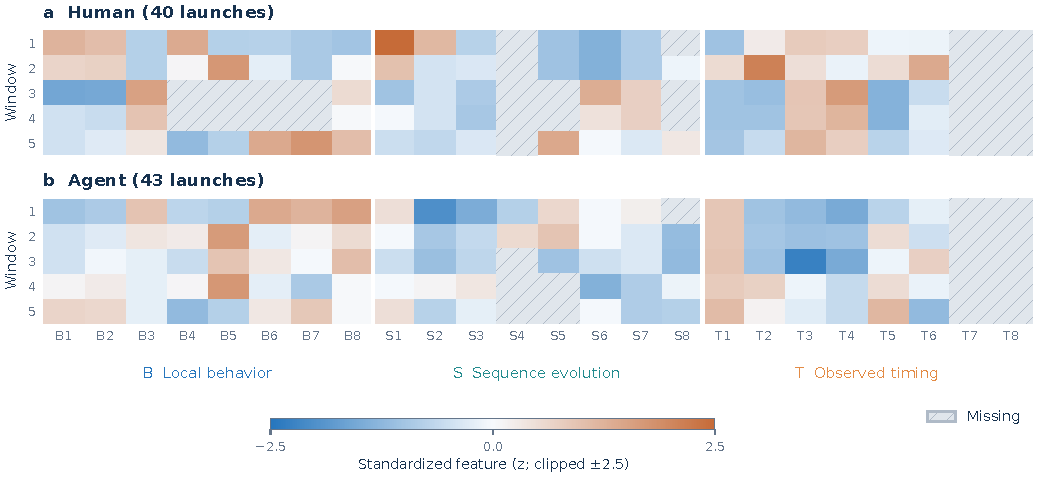
\includegraphics[width=\linewidth]{fingerprint-v2-matrix-example.pdf}
\caption{Two AIT traces from the same troubleshooting task, visualized against the 24-slot B/S/T schema over variable-length windows. T7--T8 are missing because durations are not recorded. The shared blue--amber scale shows cohort-standardized values for display. Hatched cells mark missing observations.}
\label{fig:matrix}
\end{figure}

\begin{figure}[!htbp]
\centering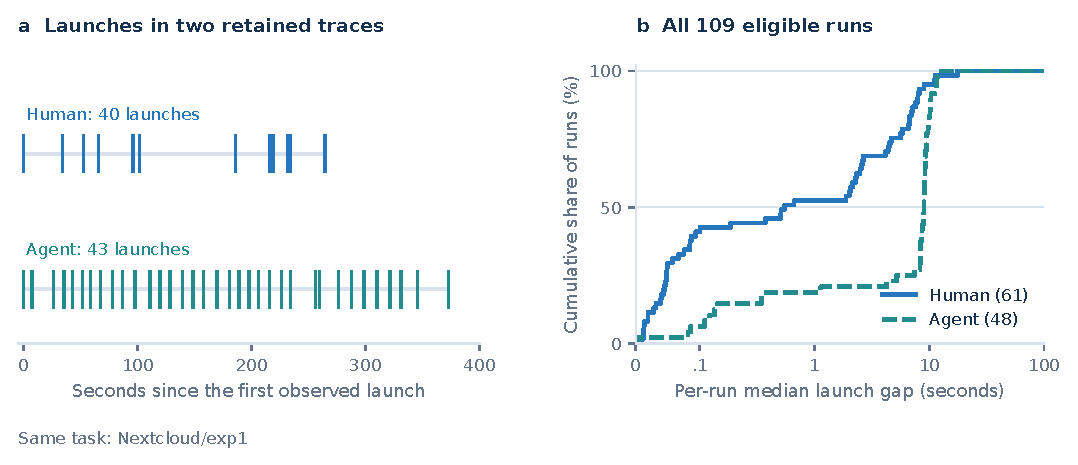
\includegraphics[width=\linewidth]{fingerprint-observed-rhythm.pdf}
\caption{Observed launch-gap timing behind T1--T6. Left, real launch timestamps from the two traces in Figure~\ref{fig:matrix}, aligned to their own first observed launch with a shared seconds scale. Right, empirical distributions of one median launch gap per run over all 109 AIT runs. The scale is logarithmic above 0.1 seconds and preserves zero gaps. Each run contributes at most its first 128 login-associated events.}
\label{fig:timing}
\end{figure}

\begin{figure}[!htbp]
\centering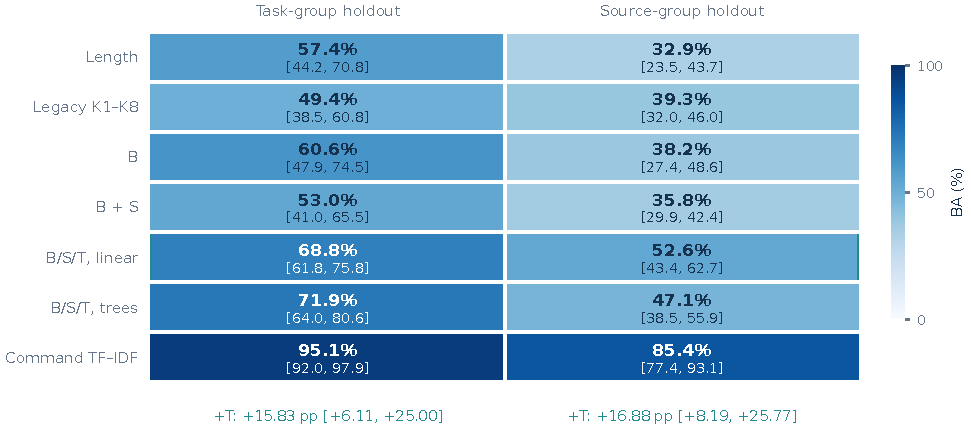
\includegraphics[width=\linewidth]{fingerprint-recognition-matrix.pdf}
\caption{Earlier execution-mode recognition on 109 AIT runs (61 Human, 48 Agent in 12 task groups). Cells report balanced accuracy and 95\% intervals for the recorded mode label. The outlined row shows the linear B/S plus six launch-gap feature readout; the bottom annotations show its paired T1--T6 increment. Collection workflow co-varies with the released labels.}
\label{fig:recognition}
\end{figure}

\FloatBarrier
\section{Conditioned association across sources}
The within-source comparisons in Figure~\ref{fig:association-comparison} and the source-held-out comparisons in Table~\ref{tab:association-ba-v3} use the conditioned shallow-tree protocol. The frozen NYU test uses the matched learners and the CTH-trained thresholds described in Appendix~\ref{app:nyu}.

\begin{table}[ht]
\centering\compacttable
\caption{Complete source-held-out association comparison. Training uses the other sources; B/S windows contain eight events. BA is in percent; differences and unadjusted 95\% cluster intervals are in percentage points. Green/red encode improvement/decline in the point estimate; interval bounds retain the uncertainty.}
\label{tab:association-ba-v3}
\setlength{\tabcolsep}{3pt}
\begin{tabular*}{\linewidth}{@{\extracolsep{\fill}}lrrr@{}}
\toprule Test source & Evidence & + B/S & $\Delta$BA [95\% CI] \\
\midrule
CTH & 51.98 & 56.69 & $\gain{+4.71}\;\textcolor{ResearchMuted}{[+0.69,+8.83]}$ \\
KYPO & 66.40 & 66.61 & $\gain{+0.21}\;\textcolor{ResearchMuted}{[-1.06,+1.36]}$ \\
Antieval & 71.90 & 68.63 & $\loss{-3.27}\;\textcolor{ResearchMuted}{[-6.28,-0.22]}$ \\
\bottomrule
\end{tabular*}
\end{table}
\begin{figure}[!htbp]
\centering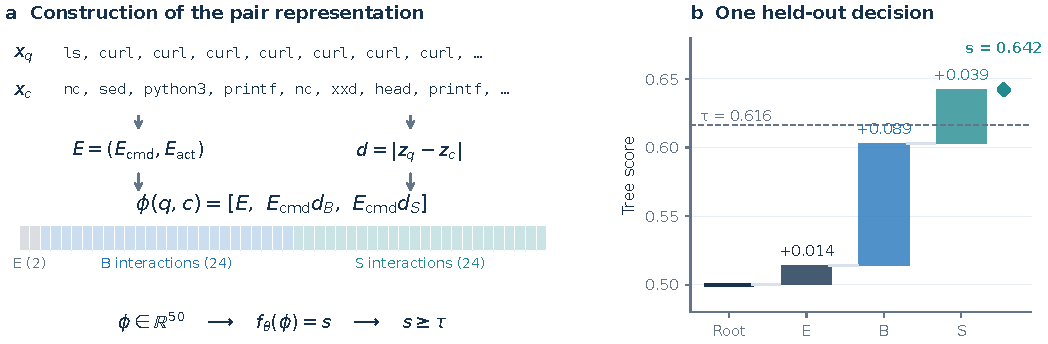
\includegraphics[width=\linewidth]{fingerprint-conditioned-association.pdf}
\caption{Earlier conditioned tree scorer and one held-out CTH \texttt{locktalk} decision. Panel a shows how two evidence scores and 48 conditioned B/S differences enter the scorer. Panel b shows contributions to a selected score among 31 corrected cross-mode same-task pairs in the purged source holdout. Each model uses its own training-selected threshold.}
\label{fig:conditioned-association}
\end{figure}

\begin{figure}[!htbp]
\centering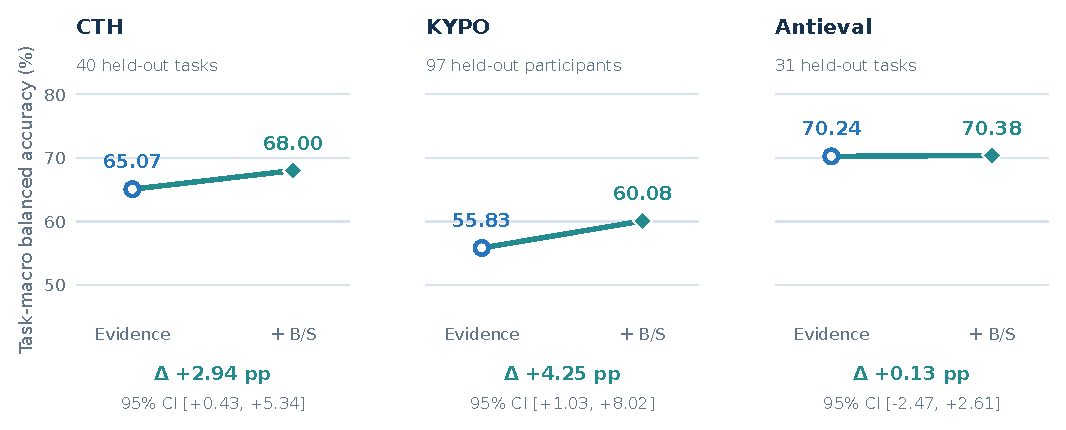
\includegraphics[width=\linewidth]{fingerprint-association-comparison.pdf}
\caption{Earlier within-source evidence-conditioned association. Panel a compares the same shallow-tree family before and after adding B/S. Panel b shows paired BA changes and 95\% intervals. CTH and Antieval resample tasks. KYPO resamples query participants with galleries fixed. The intervals are exploratory and unadjusted.}
\label{fig:association-comparison}
\end{figure}

\end{document}
